\documentclass{article}
\usepackage{v-problem}
\renewcommand{\ans}{\quad}
\vgeometry

\begin{document}
\vtitle[ROTATION]

\def\pn{03}
\def\book{BOOK}
\def\page{2022}
\def\gdrive{https://drive.google.com/drive/folders/1Z2xH8aM2FbhaHSK0OYItSEdgMeFFCEV5?usp=share_link}

\def\question{
A homogeneous solid cylinder roller of radius $R$ and mass $m$ is pulled on a cricket pitch by a horizontal force. Assuming rolling without slipping, angular acceleration of the cylinder is
}
\def\option{
\begin{tasks}(2)
	\task $\dfrac{F}{2mR}$
	\task $\dfrac{2F}{3mR}$ \ans
	\task $\dfrac{3F}{2mR}$ 
	\task $\dfrac{F}{3mR}$
\end{tasks}
}

\vspace*{\fill}
\begin{tikzpicture}
	\node[qnumber] (n) at (0, 0)[scale=2] {$\pn.$};
	\node[question] (q) [right=2mm of n.east] {\question};
	\tzline[divider]<-0.125, 0> (q.north west)(q.south west);
	%\node[format] (f) at  (q.south east){[\book \quad \page]};
\end{tikzpicture}	
\vspace*{\fill}

\begin{center}
	\begin{tikzpicture}
		\tzcoor*(0,1)(O)
		\pic at (0, 0) {frame=7cm};
		\tzcircle(O)(1)
		\tzline+[->](O)(2, 0){$F$}[r]	
		\tzarc[->](O)(150:30:1.25){$\alpha$}[r]
	\end{tikzpicture}
\end{center}
\vspace*{\fill}

\begin{tikzpicture}
\node[minimum width=1cm](n) at (0, 0){}; 
\node[option, anchor=west] at (n.east){\option};
\end{tikzpicture}

\vspace*{\fill}
\pagebreak


\vtitle[\texttt{Solution}]

$\Rightarrow$
\begin{center}
\begin{tikzpicture}
	\tzcoor*(0,1)(O)
	\tzcircle(O)(1)
	\tzline+[->](O)(2, 0){$F$}[r]	
	\tzarc[->](O)(150:30:1.25){$\alpha$}[r]	
	\tzline+[->]($(O)+(0, -1)$)(-2, 0){$f_r$}[l]
\end{tikzpicture}
\end{center}
\begin{align*}
	\intertext{Torque due to friction($f_r$) about the center of the cylinder is zero.}
	\tau &= I\alpha\\
	f_rR &= \dfrac{1}{2}mR^2\alpha\\
	f_r &= \dfrac{1}{2}mR\alpha\\
	\intertext{Net force on the cylinder is $F-f_r$.}
	\Rightarrow F-f_r &= ma\\
	\Rightarrow F-\dfrac{1}{2}mR\alpha &= mR\alpha\\
	\Rightarrow \alpha &= \dfrac{2F}{3mR}
\end{align*}
\begin{align*}
	\intertext{Alternatively, using IAR(Instantaneous Axis of Rotation)}
	\intertext{Lets assume the cylinder is rotating about the point of contact with the ground.}
	\tau &= I\alpha\\
	FR &= \dfrac{3}{2}mR^2\alpha\\
	\alpha &= \dfrac{2F}{3mR}
\end{align*}
\pagebreak

\vspace*{\fill}
\begin{center}
	\fbox{\qrcode[height=2cm]{\gdrive}}
\end{center}
\vspace*{\fill}

\end{document}

	